\documentclass[pdf]{beamer}
\mode<presentation>{}
\usepackage{minted}
\usepackage{tikz}
\usepackage{pgffor} %% gives looping with \foreach
\usepackage[absolute,overlay]{textpos}
\usepackage{lmodern} %% scalable latin characters
\usetikzlibrary{arrows,shapes,backgrounds}
\usepackage{multirow}
\usepackage{listings} %% another package for code related stuff

%% stuff for minted
\definecolor{mintedBg}{rgb}{0.95, 0.95, 0.95}
\definecolor{blockBg}{rgb}{0.6, 0.6, 0.95}
\definecolor{rnaColor}{rgb}{0, 0.6, 0}
\definecolor{cdsColor}{rgb}{0, 0.4, 0.4}
\definecolor{rnaPol}{rgb}{0.8,0,0.8}
\definecolor{ribosomeCol}{rgb}{0.5,0.5,0.1}
\definecolor{protColor}{rgb}{0.6,0,0.6}
%% colours for nucleotides:
\definecolor{dACol}{rgb}{0.5, 0.5, 0}
\definecolor{dCCol}{rgb}{0.8, 0, 0}
\definecolor{dGCol}{rgb}{0, 0.8, 0}
\definecolor{dTCol}{rgb}{0, 0, 0.8}

\definecolor{navy}{rgb}{0, 0, 0.6}
\definecolor{pur}{rgb}{0, 0, 0.6}
\definecolor{pyr}{rgb}{0.6, 0, 0.2}

\definecolor{purple1}{rgb}{1.0, 0, 0.6}
\definecolor{purple2}{rgb}{0.8, 0, 0.8}
\definecolor{purple3}{rgb}{0.6, 0, 1.0}
%% define styles for different codes
\newminted{cpp}{linenos, bgcolor=blockBg, fontsize=\footnotesize}
%% then use \begin{cppcode}
\newminted{c}{linenos, bgcolor=mintedBg, fontsize=\footnotesize}
\newminted{perl}{linenos, bgcolor=mintedBg, fontsize=\footnotesize}

%% a command to define a subheading
\newcommand\subHeading[1]{
  \par\bigskip {\Large\bfseries#1}\par\smallskip
}

%% I detest indentation in footnotes etc, so try this:
\makeatletter
\renewcommand\@makefntext[1]{\noindent\makebox[0em][r]{\@makefnmark}\tiny#1}
\makeatother
%% the makeatletter and makeatother are required to allow me to
%% to change the macro beginning with an @. (though when I call it
%% I don't use the @ ... 

\setlength\parskip{0.5em}
\setlength\parindent{0ex}

%% to have footnotes without references. This from tex.stackexchange.com
\newcommand\blfootnote[1]{%
  \begingroup  %% this makes it a local redefinition
  \renewcommand\thefootnote{}\footnote{#1}%
  \addtocounter{footnote}{-1}  % this adjusts the footnote counter
  \endgroup
}


%% to draw a pair of genes..
\newcommand{\genePair}[3][]{
        \draw [-,#1] (#2-1,#3) -- (#2+1,#3);
        \draw [-,line width=2, purple1] (#2-0.5,#3) -- (#2+0.5,#3);
        \draw [-,#1] (#2-1,#3-0.5) -- (#2+1,#3-0.5);
        \draw [-,line width=2, purple3] (#2-0.5,#3-0.5) -- (#2+0.5,#3-0.5);  
}

\title{Multiple alignment}
\subtitle{aligning several sequences}
\author{Martin Jakt}

\begin{document}

\begin{frame}
  \titlepage
\end{frame}

\begin{frame}{Multiple Alignment. Why?}
  More natural than pairwise alignment since no reason to
  believe that similar sequences come in pairs.
  \pause
  \begin{description}
  \item[Orthologues] Sequence groups that are homologous across species
    (i.e. same gene, but different species).
  \item[Paralogues] Sequence groups that are homogolous within species
    (i.e. several genes within a species that share an evolutionary origin).
  \end{description}
  \pause

  There are usually lots of these. Hence multiple alignment is a more 'natural'
  than simple pairwise alignment.  
\end{frame}

\begin{frame}{Homology, Orthology, Paralogy}
  \begin{figure}[ht]
    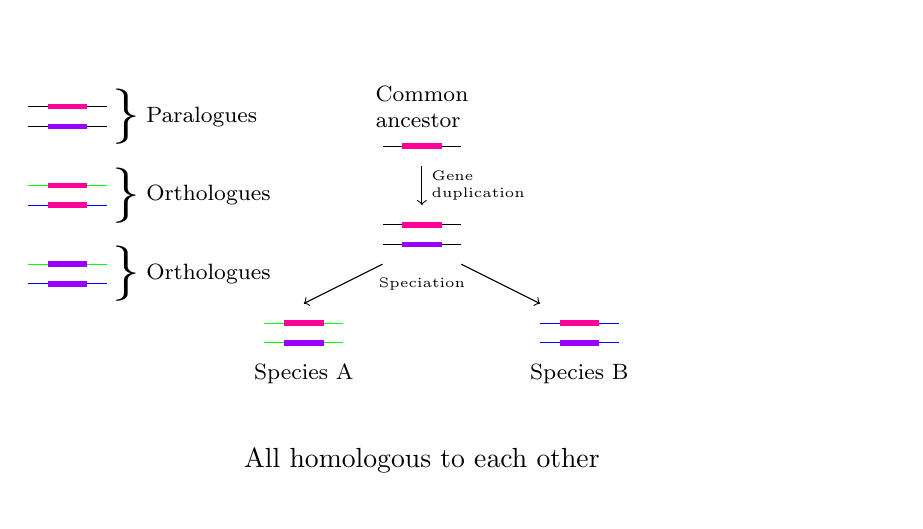
\begin{tikzpicture}[scale=0.5]
      \draw [help lines, opacity=0] (0,0) grid (22,12);
%     \foreach \x in {1,2,...,19} \node [font=\small] at (\x,0) {\x};
%     \foreach \y in {1,2,...,12} \node [font=\small] at (20,\y) {\y};
      \visible<2->{
        \node [align=left, font=\footnotesize] at (10,10) {Common\\ancestor};
        \draw [-] (9,9) -- (11,9);
        \draw [-,line width=2, purple1] (9.5,9) -- (10.5,9);
      }
      \visible<3->{
        \draw [->] (10,8.5) -- (10,7.5) node [midway, right, align=left, font=\tiny] 
        {Gene\\duplication};
        \genePair{10}{7}
      }
      \visible<4->{
        \draw [->] (9,6) -- (7,5);
        \draw [->] (11,6) -- (13,5);
        \node [font=\tiny] at (10,5.5) {Speciation};
        \genePair[green]{7}{4.5}
        \genePair[blue]{14}{4.5}
        \node [font=\footnotesize] at (7,3.2) {Species A};
        \node [font=\footnotesize] at (14,3.2) {Species B};
      }
      \visible<5->{
        \genePair{1}{10};
        \node [scale=2] at (2.5,9.75) {\}};
        \node [right, font=\footnotesize] at (2.75, 9.75) {Paralogues};
      }
      \visible<6->{
        \draw [-,green] (0,8) -- (2,8);
        \draw [-,blue] (0,7.5) -- (2,7.5);
        \draw [-,purple1, line width=2] (0.5,8) -- (1.5,8);
        \draw [-,purple1, line width=2] (0.5,7.5) -- (1.5,7.5);
        \node [scale=2] at (2.5,7.75) {\}};
        \node [right, font=\footnotesize] at (2.75,7.75) { Orthologues };
        
        \draw [-,green] (0,6) -- (2,6);
        \draw [-,blue] (0,5.5) -- (2,5.5);
        \draw [-,purple3, line width=2] (0.5,6) -- (1.5,6);
        \draw [-,purple3, line width=2] (0.5,5.5) -- (1.5,5.5);
        \node [scale=2] at (2.5,5.75) {\}};
        \node [right, font=\footnotesize] at (2.75,5.75) { Orthologues };
      }
      \visible<7->{
        \node at (10,1) {All homologous to each other};
      }
    \end{tikzpicture}
  \end{figure}
\end{frame}

\begin{frame}{Multiple Alignment. More whys}
  Addresses many biological questions and technical issues:
  \begin{itemize}
  \item diagnostic patterns for protein families
  \item detect or demonstrate homology between sequences
  \item help predict secondary and tertiary structures
  \item to suggest oligonucleotide primers for PCR
  \item essential prelude to molecular evolutionary analysis
  \item ...
  \end{itemize}
  \blfootnote{Shamelessly copied from Thompson et al., NAR 1994 22(22): 4673-4680\\
    \url{http://www.ncbi.nlm.nih.gov/pmc/articles/PMC308517/}
  }
\end{frame}

\begin{frame}{How to align many sequences?}
  In theory, possible to use dynamic programming algorithms (eg. Needleman-Wunsch,
  Smith Waterman) to find optimal alignments.

  But the complexity of these scale by $l^n$ (where $l$ is the length of the sequences,
  and $n$ is the number of sequences). Too complex both in terms of memory requirements
  processing time for more than a few sequences. (But examples exist).

  \textcolor{navy}{\emph{Heuristic}} methods are used instead. These do not guarantee an
  optimal result, but provide sufficient speed.

  Many methods exist: we will look in detail at one of these.
\end{frame}

\begin{frame}{ClustalW}
  \begin{figure}[ht]
    \includegraphics[width=0.9\textwidth]{images/clustalw_title}
  \end{figure}
\end{frame}

\begin{frame}{Why ClustalW}
  \begin{itemize}
    \item One of the most widely used methods
    \item Easy to understand
    \item Includes phylogenetic analysis
    \item Paper describes the heuristic process nicely (eg. this can be a 
      problem, so we tweaked this part of the method to give nicer results).
    \item The method extends naturally from pairwise alignment.
  \end{itemize}

\end{frame}

\begin{frame}{The clustal method}
  For a collection of sequences:
  \begin{enumerate}
  \item Align all pairs of sequences and calculate a distance matrix (table).
  \item Use the distance matrix to calculate a guide tree.
  \item Align the sequences progressively according to the branch order
    of the guide tree.
  \end{enumerate}
\end{frame}

\begin{frame}{Pairwise alignment}
  Global alignment of all pairs using a modification of Needleman-Wunsch,
  or a faster k-tuple based heuristic method.

  Scores are calculated as: number of identities / number of residues compared
  (gap positions are excluded).

  $\Rightarrow$ distances (1 - score). (no correction for multiple substiutions).
  
  This gives an n by n distance matrix. (make a figure for this).
\end{frame}

\begin{frame}{The guide tree}
  Tree created from the distances to represent the similarities between the
  sequences and to suggest an order for the progressive alignment. 

  Earlier versions used UPGMA. Newer version uses Neighbor joining algorithm.

  [make figure of tree]
\end{frame}

\begin{frame}{What is a tree}
  \begin{itemize}
  \item A way to represent a set of relationships (commonly distances or dis-similarities).
  \item Often obtained by hierarchical clustering methods from distances matrices (see below).
  \item Can also be obtained by maxium parsimony or maximum expectation methods.
  \item Originally developed to represent evolutionary relationships (i.e. phylogenetic trees)
  \item Now generally used to summarise N-dimensional data sets (covered later in the course).
  \end{itemize}
\end{frame}

\begin{frame}{UPGMA: the simplest tree}
  Unweighted Pair Group Method with Arithmetic Mean
  \begin{figure}[ht]
    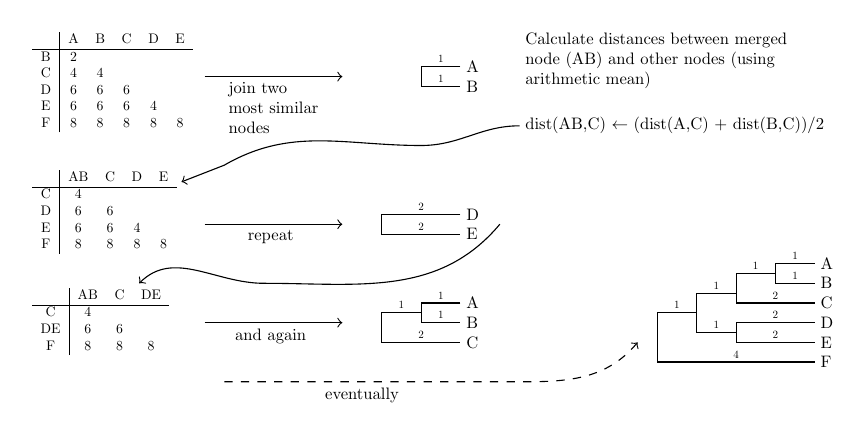
\begin{tikzpicture}[scale=0.5]
%     \draw [help lines, opacity=1] (0,0) grid (22,12);
%     \foreach \x in {1,2,...,19} \node [font=\small] at (\x,0) {\x};
%     \foreach \y in {1,2,...,12} \node [font=\small] at (20,\y) {\y};
     
     \node [below right, scale=0.5] at (0,12) {
       \begin{tabular}{ c| ccccc }
         & A & B & C & D & E \\
         \hline
         B & 2 &&&& \\
         C & 4 & 4 &&& \\
         D & 6 & 6 & 6 && \\
         E & 6 & 6 & 6 & 4 & \\
         F & 8 & 8 & 8 & 8 & 8 
       \end{tabular}
     };
     \visible<2->{
       \draw [->] (4.5,10.75) -- (8,10.75) node [midway, below, align=left, scale=0.6]
       { join two\\most similar\\nodes };
       \draw [-] (11,11) node [right, scale=0.6] {A} -- (10,11) node [midway, above, scale=0.4] {1}
       -- (10,10.5) -- (11,10.5) node [midway, above, scale=0.4] {1};
       \node [right, scale=0.6] at (11,10.5) {B};
     }
     \visible<3->{
       \node [below right, align=left, scale=0.6, text width=6cm] at (12.5,12) {
         Calculate distances between merged node (AB) and other nodes (using arithmetic mean)};
       \node [right, scale=0.6] (eq1) at (12.5,9.5) 
       {dist(AB,C) $\leftarrow$ (dist(A,C) + dist(B,C))/2};
     };         
     
     \visible<4->{
       \node [below right, scale=0.5] (mat2) at (0,8.5) {
         \begin{tabular}{ c| cccc }
           & AB & C & D & E \\
           \hline
           C & 4 &&& \\
           D & 6 & 6 && \\
           E & 6 & 6 & 4 & \\
           F & 8 & 8 & 8 & 8 
         \end{tabular} };
       \draw [->] (eq1) to [out=180,in=0] (10,9) 
       to [out=180,in=30] (5,8.5) -- (mat2); 
     }
     \visible<5->{
       \draw [->] (4.5,7) -- (8,7) node [midway, below, align=left, scale=0.6]
       { repeat };
       \draw [-] (11,7.25) node [right, scale=0.6] {D} -- (9,7.25) node [midway, above, scale=0.4] {2}
       -- (9,6.75) -- (11,6.75) node [midway, above, scale=0.4] {2};
       \node [right, scale=0.6] at (11,6.75) {E};
     }
     \visible<6->{
       \node [below right, scale=0.5] (mat3) at (0,5.5) {
         \begin{tabular}{ c| ccc }
           &  AB & C & DE \\
           \hline
           C  & 4 && \\
           DE & 6 & 6 & \\
           F  & 8 & 8 & 8 
         \end{tabular} };
       \draw [->] (12,7) to [out=230,in=0] (6,5.5) to [out=180,in=45] (mat3);
     }
     \visible<7->{
       \draw [->] (4.5,4.5) -- (8,4.5) node [midway, below, align=left, scale=0.6]
       { and again };
       \draw [-] (11,5) node [right, scale=0.6] {A} -- (10,5) node [midway, above, scale=0.4] {1}
       -- (10,4.5) -- (11,4.5) node [midway, above, scale=0.4] {1};
       \node [right, scale=0.6] at (11,4.5) {B};
       \draw [-] (10,4.75) -- (9,4.75) node [midway, above, scale=0.4] {1}
       -- (9,4) -- (11,4) node [midway, above, scale=0.4] {2};
       \node [right, scale=0.6] at (11,4) {C};
     }
     \visible<8->{
       \draw [->, dashed] (5,3) -- (12,3) node [pos=0.5, below, scale=0.6] {eventually}
       to [out=0,in=230] (15.5,4);
       \draw [-] (20,6) node [right, scale=0.6] {A} -- (19,6) node [midway, above, scale=0.4] {1}
       -- (19,5.5) -- (20,5.5) node [midway, above, scale=0.4] {1};
       \node [right, scale=0.6] at (20,5.5) {B};
       \draw [-] (19,5.75) -- (18,5.75) node [midway, above, scale=0.4] {1}
       -- (18,5) -- (20,5) node [midway, above, scale=0.4] {2};
       \node [right, scale=0.6] at (20,5) {C};
       \draw [-] (18,5.25) -- (17,5.25) node [midway, above, scale=0.4] {1}
       -- (17,4.25) -- (18,4.25) node [midway, above, scale=0.4] {1}
       -- (18,4.5) -- (20,4.5) node [midway, above, scale=0.4] {2};
       \draw (20,4) -- (18,4) node [midway, above, scale=0.4] {2} -- (18,4.25);
       \draw (17,4.75) -- (16,4.75) node [midway, above, scale=0.4] {1}
       -- (16,3.5) -- (20,3.5) node [midway, above, scale=0.4] {4};
       \node [right, scale=0.6] at (20,4.5) {D};
       \node [right, scale=0.6] at (20,4) {E};
       \node [right, scale=0.6] at (20,3.5) {F};
     }
   \end{tikzpicture}
 \end{figure}
\end{frame}

\begin{frame}{Neighbor joining algorithm}
  \begin{itemize}
  \item Basic method similar to UPGMA
  \item Modified distance matrix used to find nearest nodes to join
  \item Distances of pair members to joins are influenced by distances to external nodes
  \item Does not assume equal rate of evolution ($\Rightarrow$) neighbours have
    differeing lengths to their joining nodes.
  \item Better than UPGMA
  \end{itemize}
\blfootnote{Saitou and Nei, Mol Biol Evol 1987, Jul;4(4);406-25}  
\end{frame}

\begin{frame}{Neighbor joining algorithm}
  Nodes to be joined (i.e. neighbors) are chosen from a Q matrix:
  $$
  Q_{i,j} = (n-2)d_{i,j} - \sum_{k=1}^n{d_{i,k}} - \sum_{k=1}^n{d_{j,k}}
  $$
  Where $d_{i,j}$ is the distance between the $i^th$ and $j^th$ nodes, n is
  the total number of nodes.\\
  This will preferentially select outliers to join (i.e. pairs of nodes
  which are distant from the larger set).
\end{frame}

\begin{frame}{Neighbor joining (2)}
  The pair with the lowest $Q$ value are joined by a new node. If we refer to the
  neighbors as $f$ and $g$, and the new node as $u$, then we calculate the distance
  to the new node as follows:
  $$
  \delta(f,u) = \frac{1}{2}d_{f,g} + \frac{1}{2(n-2)}\big[ \sum_{k=1}^n{d_{f,k}} - \sum_{k=1}^n{d_{g,k}} \big]
  $$
\end{frame}

\begin{frame}{Progressive alignment}
  How to align two alignments?
  
  Modify the scoring function to use several sequences.
\end{frame}

\begin{frame}{Refinements}

\end{frame}

\end{document}

